% ------------------------------------------------------------------------------
% TYPO3 CMS 7.2 - What's New - Chapter "Introduction" (English Version)
%
% @author	Michael Schams <schams.net>
% @license	Creative Commons BY-NC-SA 3.0
% @link		http://typo3.org/download/release-notes/whats-new/
% @language	English
% ------------------------------------------------------------------------------
% LTXE-CHAPTER-UID:		16517900-07a67f43-fe9f3e35-7e924788
% LTXE-CHAPTER-NAME:	Introduction
% ------------------------------------------------------------------------------

\section{Uvod}
\begin{frame}[fragile]
	\frametitle{Uvod}

	\begin{center}\huge{Uvod}\end{center}
	\begin{center}\huge{\color{typo3darkgrey}\textbf{Cinjenice}}\end{center}

\end{frame}

% ------------------------------------------------------------------------------
% LTXE-SLIDE-START
% LTXE-SLIDE-UID:		dce36242-c42d3b1a-9256338c-7ba3f3b9
% LTXE-SLIDE-ORIGIN:	6d5e9f3e-f9d9677e-43d7d497-e80ba9ef English
% LTXE-SLIDE-TITLE:		TYPO3 CMS 7.2 - The Facts
% ------------------------------------------------------------------------------
\begin{frame}[fragile]
	\frametitle{Uvod}
	\framesubtitle{TYPO3 CMS 7.2 - Cinjenice}

	\begin{itemize}
		\item Datum objavljivanja: 28. april 2015.
		\item Tip objavljivanja: "Brza objava" ("Sprint Release")
		\item Vizija: Prihvatiti, inovirati, dostaviti
		\item Glavni fokus: Korisnicki interfejs
	\end{itemize}

	\begin{figure}
		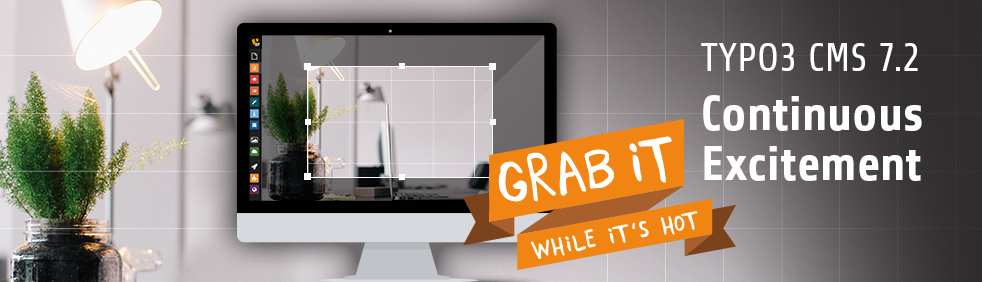
\includegraphics[width=0.95\linewidth]{Introduction/typo3cms72-teaser.png}
	\end{figure}

\end{frame}

% ------------------------------------------------------------------------------
% LTXE-SLIDE-START
% LTXE-SLIDE-UID:		be262c6f-e46fb037-7681e9f5-b16ddef1
% LTXE-SLIDE-ORIGIN:	759c3860-d5061f6e-2bb0009f-6ea130c8 English
% LTXE-SLIDE-TITLE:		System Requirements
% ------------------------------------------------------------------------------
\begin{frame}[fragile]
	\frametitle{Uvod}
	\framesubtitle{Sistemski zahtevi}

	\begin{itemize}
		\item PHP*:\tabto{3cm}v5.5.0 - v5.6.x
		\item MySQL:\tabto{3cm}v5.5.x - v5.6.x (no strict mode)
		\item Prostor na disku:\tabto{3cm}min 200 MB
		\item PHP podesavanja:

			\begin{itemize}
				\item memory\_limit >= 128M
				\item max\_execution\_time >= 240s
				\item opcija \texttt{--disable-ipv6} \underline{ne sme} se koristit
			\end{itemize}

		\item Administratorski interfejs zahteva IE >= 9 ili bilo koji drugi moderni pretrazivac

	\end{itemize}

	\vspace{1cm}
	*) Dodatno objasnjenje: \href{http://typo3.org/news/article/php-minimum-requirements-for-typo3-cms-7/}{PHP Minimum Requirements for TYPO3 CMS 7}

\end{frame}

% ------------------------------------------------------------------------------
% LTXE-SLIDE-START
% LTXE-SLIDE-UID:		a591867d-d1b6280a-b6f4d9e7-c592c674
% LTXE-SLIDE-ORIGIN:	70c77c41-e2b83d82-2f182996-98061070 English
% LTXE-SLIDE-TITLE:		Development And Release Timeline
% ------------------------------------------------------------------------------
\begin{frame}[fragile]
	\frametitle{Uvod}
	\framesubtitle{Vreme razvoja i datumi objavljivanja}

	\begin{figure}
		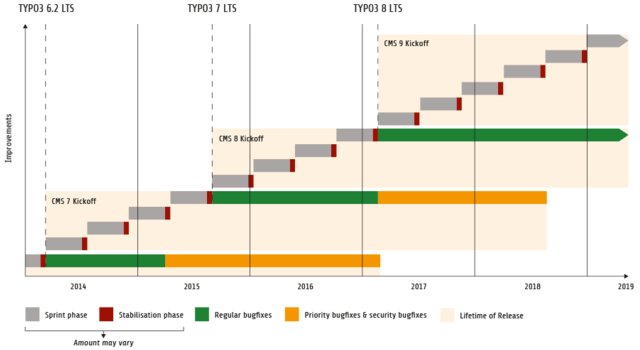
\includegraphics[width=0.90\linewidth]{Introduction/ReleaseAgenda.png}
	\end{figure}

\end{frame}

% ------------------------------------------------------------------------------
% LTXE-SLIDE-START
% LTXE-SLIDE-UID:		650837ac-b27fb921-fe403d6d-4d8c8a81
% LTXE-SLIDE-ORIGIN:	b55d3fe9-76807061-d97f3fee-7db1f190 English
% LTXE-SLIDE-TITLE:		TYPO3 CMS Roadmap
% ------------------------------------------------------------------------------
\begin{frame}[fragile]
	\frametitle{Uvod}
	\framesubtitle{TYPO3 CMS plan}

	Predvidjeni datumi objavljivanja i njihov osnovni fokus:

	\begin{itemize}
		\item v7.0 \tabto{1.0cm}02/Dec/2014\tabto{3.4cm}Remont administratorskog interfejsa prvi deo
		\item v7.1 \tabto{1.0cm}24/Feb/2015\tabto{3.4cm}Ciscenje osnove sistema i optimizacija

		\item
			\begingroup
				\color{typo3orange}
					v7.2 \tabto{1.0cm}28/Apr/2015\tabto{3.4cm}Korisnicki interfejs
			\endgroup

		\item v7.3 \tabto{1.0cm}09/Jun/2015\tabto{3.4cm}Ekosistem za dodatke, Composer\newline
			\tabto{3.4cm}i upravljanje prosirenjima
		\item v7.4 \tabto{1.0cm}04/Aug/2015\tabto{3.4cm}Remont administratorskog interfejsa drugi deo
		\item v7.5 \tabto{1.0cm}29/Sep/2015\tabto{3.4cm}\textit{(bice odredjeno...)}
		\item v7.6 \tabto{1.0cm}xx/xxx/2015\tabto{3.4cm}\textbf{TYPO3 CMS 7 LTS}\newline
			\tabto{3.4cm}(Verzija sa dugorocnom podrskom)
	\end{itemize}

	\smaller
		\url{https://typo3.org/typo3-cms/roadmap/}\newline
		\url{http://typo3.org/news/article/embrace-and-innovate-typo3-cms-7/}
	\normalsize

\end{frame}

% ------------------------------------------------------------------------------
% LTXE-SLIDE-START
% LTXE-SLIDE-UID:		120f3d6f-b2ee06ee-7729b0e0-32a6a99a
% LTXE-SLIDE-ORIGIN:	b0c28f26-c3ca2e99-195954a8-ed76f9d4 English
% LTXE-SLIDE-TITLE:		Installation
% ------------------------------------------------------------------------------
\begin{frame}[fragile]
	\frametitle{Uvod}
	\framesubtitle{Instalacija}

	\begin{itemize}
		\item Zvanicna procedura za instalaciju na Linux/Mac OS X\newline
			(DocumentRoot na primer \texttt{/var/www/site/htdocs}):
		\begin{lstlisting}
			$ cd /var/www/site
			$ wget --content-disposition get.typo3.org/7.2
			$ tar xzf typo3_src-7.2.0.tar.gz
			$ cd htdocs
			$ ln -s ../typo3_src-7.2.0 typo3_src
			$ ln -s typo3_src/index.php
			$ ln -s typo3_src/typo3
			$ touch FIRST_INSTALL
		\end{lstlisting}

		\item Simbolicki linkovi (Symbolic links) na Microsoft Windows:

			\begin{itemize}
				\item Koristiti \texttt{junction} za Windows XP/2000
				\item Koristiti \texttt{mlink} za Windows Vista i Windows 7
			\end{itemize}

	\end{itemize}
\end{frame}

% ------------------------------------------------------------------------------
% LTXE-SLIDE-START
% LTXE-SLIDE-UID:		7fe5ca06-5b7485e7-1d868a10-d1e84aa4
% LTXE-SLIDE-ORIGIN:	48136734-ae508d23-bce5811d-667f8908 English
% LTXE-SLIDE-TITLE:		Upgrade to TYPO3 CMS 7
% ------------------------------------------------------------------------------
\begin{frame}[fragile]
	\frametitle{Uvod}
	\framesubtitle{Nadogradnja na TYPO3 CMS 7.x}

	\begin{itemize}
		\item Nadogradnja je moguca samo sa TYPO3 CMS 6.2 LTS
		\item TYPO3 CMS < 6.2 bi prvo trebalo nadograditi na TYPO3 CMS 6.2 LTS
	\end{itemize}

	\begin{itemize}

		\item Upsutstvo za nadogradnju:\newline
			\smaller\url{http://wiki.typo3.org/Upgrade#Upgrading_to_7.2}\normalsize
		\item Zvanicni TYPO3 vodic "TYPO3 Installation and Upgrading":
			\smaller\url{http://docs.typo3.org/typo3cms/InstallationGuide}\normalsize
		\item Opsti pristup:
			\begin{itemize}
				\item Proveriti minimalne sistemske zahte \small(PHP, MySQL, itd.)
				\item Proveriti \textbf{deprecation\_*.log} u staroj TYPO3 instanci
				\item Nadograditi sva prosirenja na najnoviju verziju
				\item Postaviti nove fajlove i pokrenuti Install Tool \textrightarrow Upgrade Wizard
				\item Proveriti startup modul za administratore (opciono)
			\end{itemize}
	\end{itemize}

\end{frame}

% ------------------------------------------------------------------------------
